\documentclass[12pt]{article}

%===============================
%
%          📦 Paquetes
%
%===============================

\usepackage[a4paper, top=2cm, bottom=2cm, left=2.5cm, right=2.5cm]{geometry}
\usepackage[spanish]{babel}
\usepackage[utf8]{inputenc}
\usepackage{amsmath}
\usepackage{multicol}
\usepackage{graphicx}
\usepackage{hyperref}
\usepackage{booktabs}
\usepackage{pgfplots}
\pgfplotsset{compat=1.18}

\title{
  \vspace{2cm}
  \pagenumbering{gobble}
  
\includegraphics[width=5cm]{../assets/logo-utp.png} \\
  \vspace{1cm}
  \textbf{Universidad Tecnológica del Perú} \\
  \vspace{2cm}
  \textbf{Investigación Operativa} \\
  \vspace{1cm}
  \large \textbf{S03 - Ejercicios}
}
\author{
  \textbf{Torres Vara, Mateo Nicolas} - \texttt{U24308542} \\
  \texttt{Sección 36373}
}



\begin{document}
\maketitle
\begin{center}

  Docente: Alberto Andre Reyna Alcantara

\end{center}

%======================================
%
%          📚 Inicio del documento
%
%======================================

\newpage
\section*{Ejercicio 1}
\noindent Una fábrica de muebles de oficina produce dos tipos de escritorios: tipo 1 y tipo 2, los hace en su planta de producción, usando maderas de ébano, cedro y pino en unidades cuadradas con un mismo espesor, a saber: un escritorio de tipo 1 requiere 30 unidades cuadradas de ébano,12 de cedro y 45 de pino, para un escritorio de tipo 2 se requieren 60 unidades cuadradas de ébano, 48 de cedro y 30 de pino. Los escritorios producen por su venta una ganancia de S/560.00 los de tipo 1, y S/ 470.00 los de tipo 2. En la actualidad, la empresa dispone de 600unidades cuadradas de ébano, 384 de cedro y 660 de pino. Han recibido pedidos para ambostipos de escritorio, y les gustaría producir la cantidad de escritorios de los dos tipos quemaximicen la ganancia. ¿Cuántos escritorios deben producir de cada tipo? \\
\begin{center}
  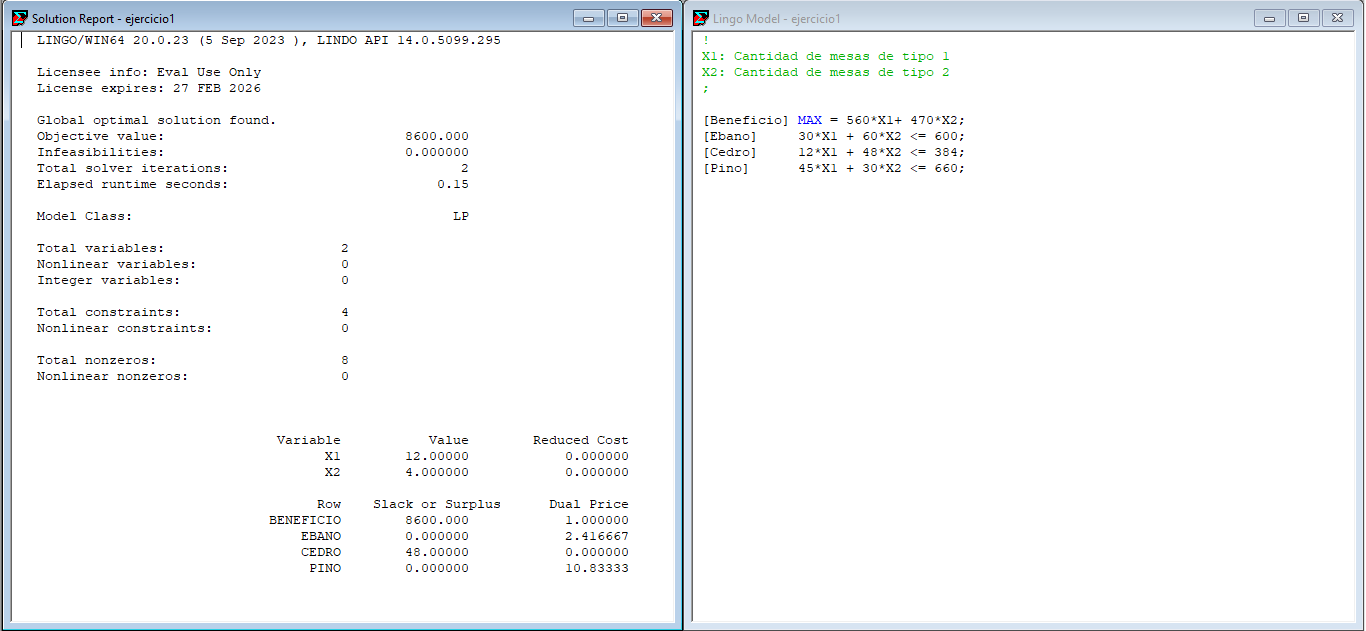
\includegraphics[width=1\textwidth]{./assets/ejercicio1.PNG}
\end{center}
\subsection*{Conclusión}
\noindent Para maximizar la ganancia se deben producir 12 mesas de tipo 1 y 4 mesas de tipo 2.



\newpage
\section*{Ejercicio 2}
\noindent Un paciente requiere una dieta estricta con dos alimentos A y B. Cada unidad del alimento A contiene 120 calorías y 2 gramos de proteínas. La unidad del alimento B contiene 100 calorías y 5 gramos de proteínas. La dieta requiere como mínimo de 1000 calorías y 30 gramos de proteínas. Si el precio de cada unidad del alimento A es de S/ 60 y de cada unidad del alimento B es de S/ 80, ¿Cuántas unidades de cada alimento debe contener la dieta para que el costo sea mínimo? \\
\begin{center}
  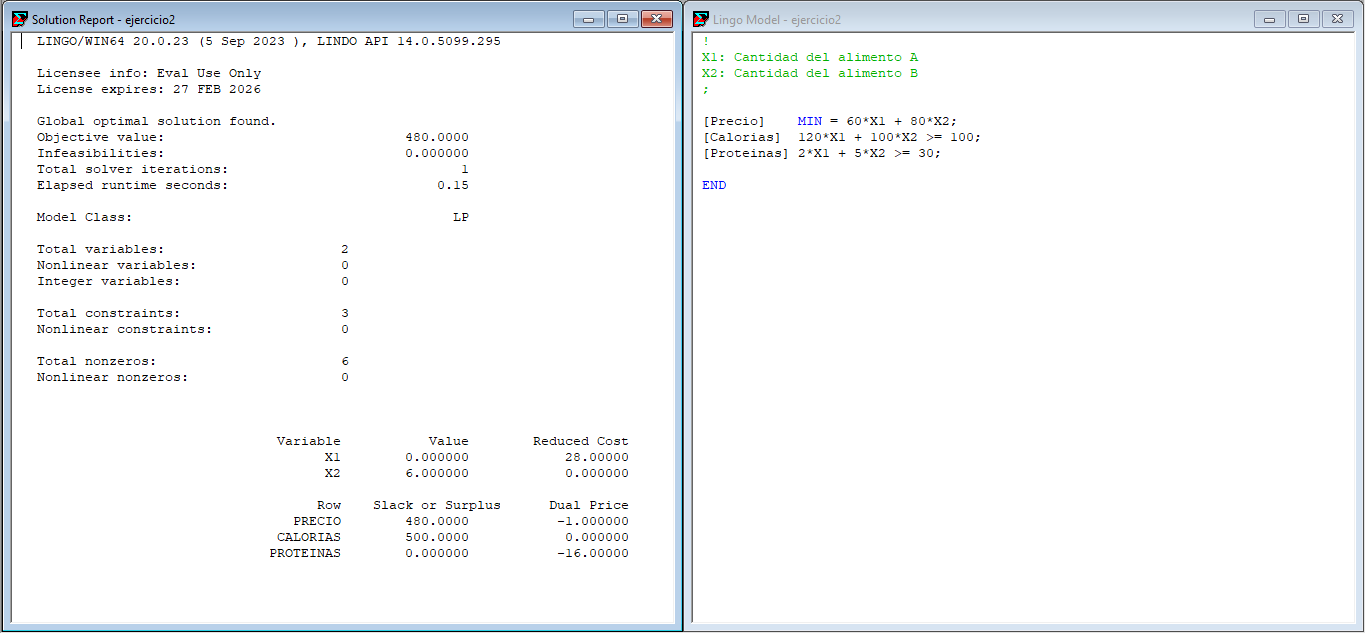
\includegraphics[width=1\textwidth]{./assets/ejercicio2.PNG}
\end{center}
\subsection*{Conclusión}
Para minimizar los costos se deben producir 0 alimentos A y 6 alimentos B



\newpage
\section*{Ejercicio 3}
\noindent Una empresa fabrica autos sedán y compactos. Los datos asociados a la producción de estos modelos se muestran a continuación, calcule:
\begin{table}[h]
  \centering
  \begin{tabular}{|c|c|c|c|}
  \hline
                            & \textbf{Puertas}  & \textbf{Mano Obra}  & \textbf{Precio Venta} \\ \hline
  Sedán                     & 4                 & 18 horas            & 12000                 \\ \hline
  Compacto                  & 2                 & 20 horas            & 8000                  \\ \hline
  \textbf{Total disponible} & 1000              & 9000                &                       \\ \hline
  \textbf{Costos Unitario}  & 500               & 70                  &                       \\ \hline
  \end{tabular}
  \caption{Variables y restricciones}
  \label{tab:Ejercicio3}
\end{table}

\begin{center}
  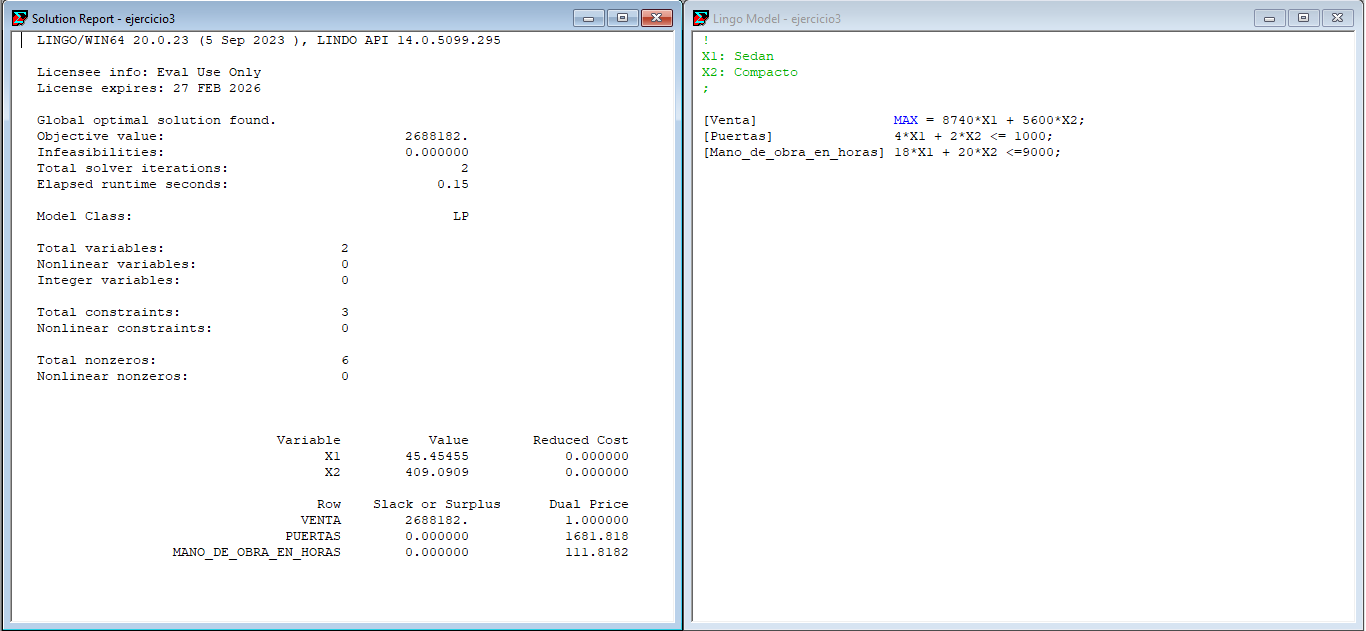
\includegraphics[width=1\textwidth]{./assets/ejercicio3.PNG}
\end{center}

\newpage
\section*{Recursos y créditos}

\begin{itemize}
    \item \textbf{Código fuente:} \href{https://github.com/MateoTVara/C08-InvestigacionOperativa}{Repositorio GitHub - Investigación Operativa}
    \item \textbf{Carátula por:} \href{https://github.com/1nfinit0}{1nfinit0 en GitHub}
\end{itemize}

\end{document}